\documentclass[runningheads]{llncs}
\usepackage{graphicx}
\usepackage[width=122mm,left=12mm,paperwidth=146mm,height=193mm,top=12mm,paperheight=217mm]{geometry}
\usepackage{amsmath,amssymb} % define this before the line numbering.

\DeclareMathOperator*{\argmin}{argmin}

%\usepackage{ruler}
\usepackage{color}

%\documentclass{llncs}
%\usepackage{graphicx}
%\usepackage{geometry}
%\geometry{margin=2cm}
%\usepackage{amsmath}

\usepackage{pgfplots}
\usepackage{filecontents}
\usepackage[caption=false]{subfig}
\usepackage{listings}
\lstset{
basicstyle=\small\ttfamily,
columns=flexible,
breaklines=true
}

\begin{document}
\title{Dissecting Neural Style Transfer}
\author{Xi Du}
\institute{Australian National University, Australia\\
\email{u6559090@anu.edu.au}}
\maketitle 
\begin{abstract}
\cite{method}

\keywords{Neural network, Deep learning, 
Small data, Interpretability .}
\end{abstract}

\section{Introduction}

\section{Literature Review}

\section{Method}

\subsection{Deep Neural Network}

For the purpose of implementing and even extending neural style transfer algorithms,
it is not necessary to understand how a neural network is trained, because
we can use pretrained model for example vgg19 \cite{vgg19}.

It is necessary to point out that a deep neural network that neural style transfer
is concerend about
is just a sequence of functions
$F_1,F_2,F_3,...$
whose inputs and outputs are all multi-dimensional arrays, as illustrated in Figure \ref{f1f2f3}.
\begin{figure}
\center
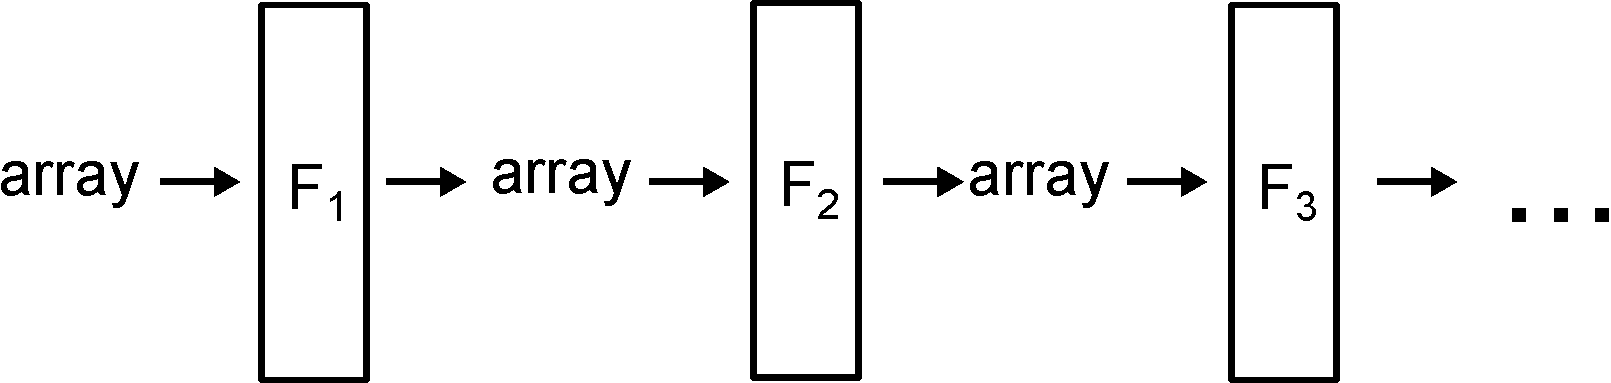
\includegraphics[width=0.6\textwidth]{f1f2f3.pdf}
\caption{A deep neural network \label{f1f2f3}}
\end{figure}
Because the arrays have usually more than two numbers of dimensions
they are not really matrices.
The arrays are called tensors (as in TensorFlow or torch.Tensor in PyTorch) 
but actual tensor algebra in a mathematical sense is rarely relevant.
The functions need to be differentiable, which is handled automatically by modern 
deep learning frameworks.
Other than that we can treat the functions as blackboxes because we are 
not concerned of training the model.
A ``layer'' in a deep neural network refers to a few consecutive functions together.
It is not particularly necessary to consider ``layers'' in this work. 
Though it is important to note that in our illustrations there are functions instead of layers.

\subsection{vgg19 model}
For the vgg19 model that most neural style transfer implementations available are based on,
The inputs and outpus of each function are all arrays with 4 dimensions.
The word ``dimension'' here may mean something slightly different from what ``dimension'' means in
for example ``$3$-dimension vector''. 
Some people call the number of dimensions ``rank'' which would then raise another confusion with the rank of matrices.
We give an illustration for the vgg19 model in Figure \ref{vgg512}
\begin{figure}
\center
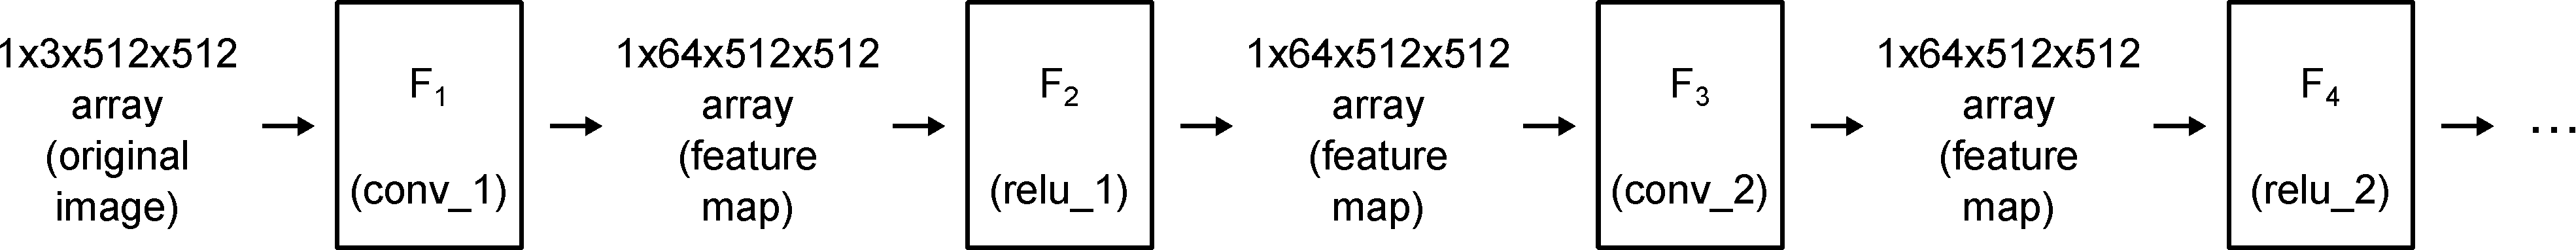
\includegraphics[width=\textwidth]{vgg512.pdf}
\caption{The VGG19 model with an $512\times512$ RGB image as its input \label{vgg512}}
\end{figure}

The 1st dimension is the ``batch'' dimension, which means that you can put several images through the
series of functions.
In neural style transfer implementations it is usually just one image each time.
So the 1st dimension is always 1, even between the $F$ functions, throughout this work.

The 2nd dimension is the ``feature'' dimension. For a raw RGB image, it is 3.
Intermediate arrays between, for example, $F_3$ and $F_4$, usually 
have a size much larger than 3, such as 64 or 128.

The 3nd and 4th dimensions are just spatial locations. 
For a $512\times512$ image they are 512 and 512. 
For intermediate arrays, these 2 dimensions are sometimes scaled down
to half or even $\frac{1}{4}$ of the sizes of the image. 
The functions $F_1,F_2,F_3,...$ now have meaningful names such as relu\_1, conv\_2 now.

The arrays after the initial image are called \emph{feature maps}, because their value means
``how much a feature x exists at position y and x''.
Take a $1\times64\times512\times512$ feature map for example. There are 64 types of features.
Its [1, 17, 111, 222] element, would then refer to the extent that the 17th type feature exists
at the position of the 222th column of the 111th row. This ``extent'' could also be negative.

\subsection{Vanilla neural style transfer}

The vanillay neural style transfer algorithm \cite{nst} is 
structured as iteratively solving an optimisation problem.
The argument to optimise is the image as a multidimensional array,
of size $1\times3\times512\times512$ for example.
The interative solver can be many, but in our case it is 
L-BFGS.It is an optimisation methodology that approximates the BFGS (Broyden - 
Fletcher - Goldfarb - Shanno) algorithm using optimal amount of system 
memory. This algorithm is famous for estimating the parameters in Machine 
Learning domain occupying only linear space for performing the computation. 
The main goal of L-BFGS is to minimize the differentiable scalar function f(x)
over the non-constrained values of  a real valued vector (x). 
 
The initial value of the argument could be either white noise or the content image,
but the latter appeared to make the optimisation much easier.

The key issue here is still how to structure the optimisation target.
The value to minimise is a linear combination of a ``style loss'' 
and ``content loss''.
Although these appeared to be two weights,
actually only their ratio mattered.
We simply fixed the weight of the content loss to 1 and
leave the weight of the style loss as a adjustable hyperparameter $k$.
\begin{align}
\argmin\limits_{\text{image}} (kL_\text{style}+L_\text{content})
\end{align}

The content loss $L_\text{content}$ is the easier one to explain of the two losses.
It is the mean square error between the outputs of a certain function in the
vgg19 taking the current argument image and the content image as inputs respectively.
We say ``a certain'' function because the output of which function to choose is
adjustable.
A typical choice is the output of \verb|conv_4| function. See Figure \ref{contentloss}.
\begin{figure}
\center
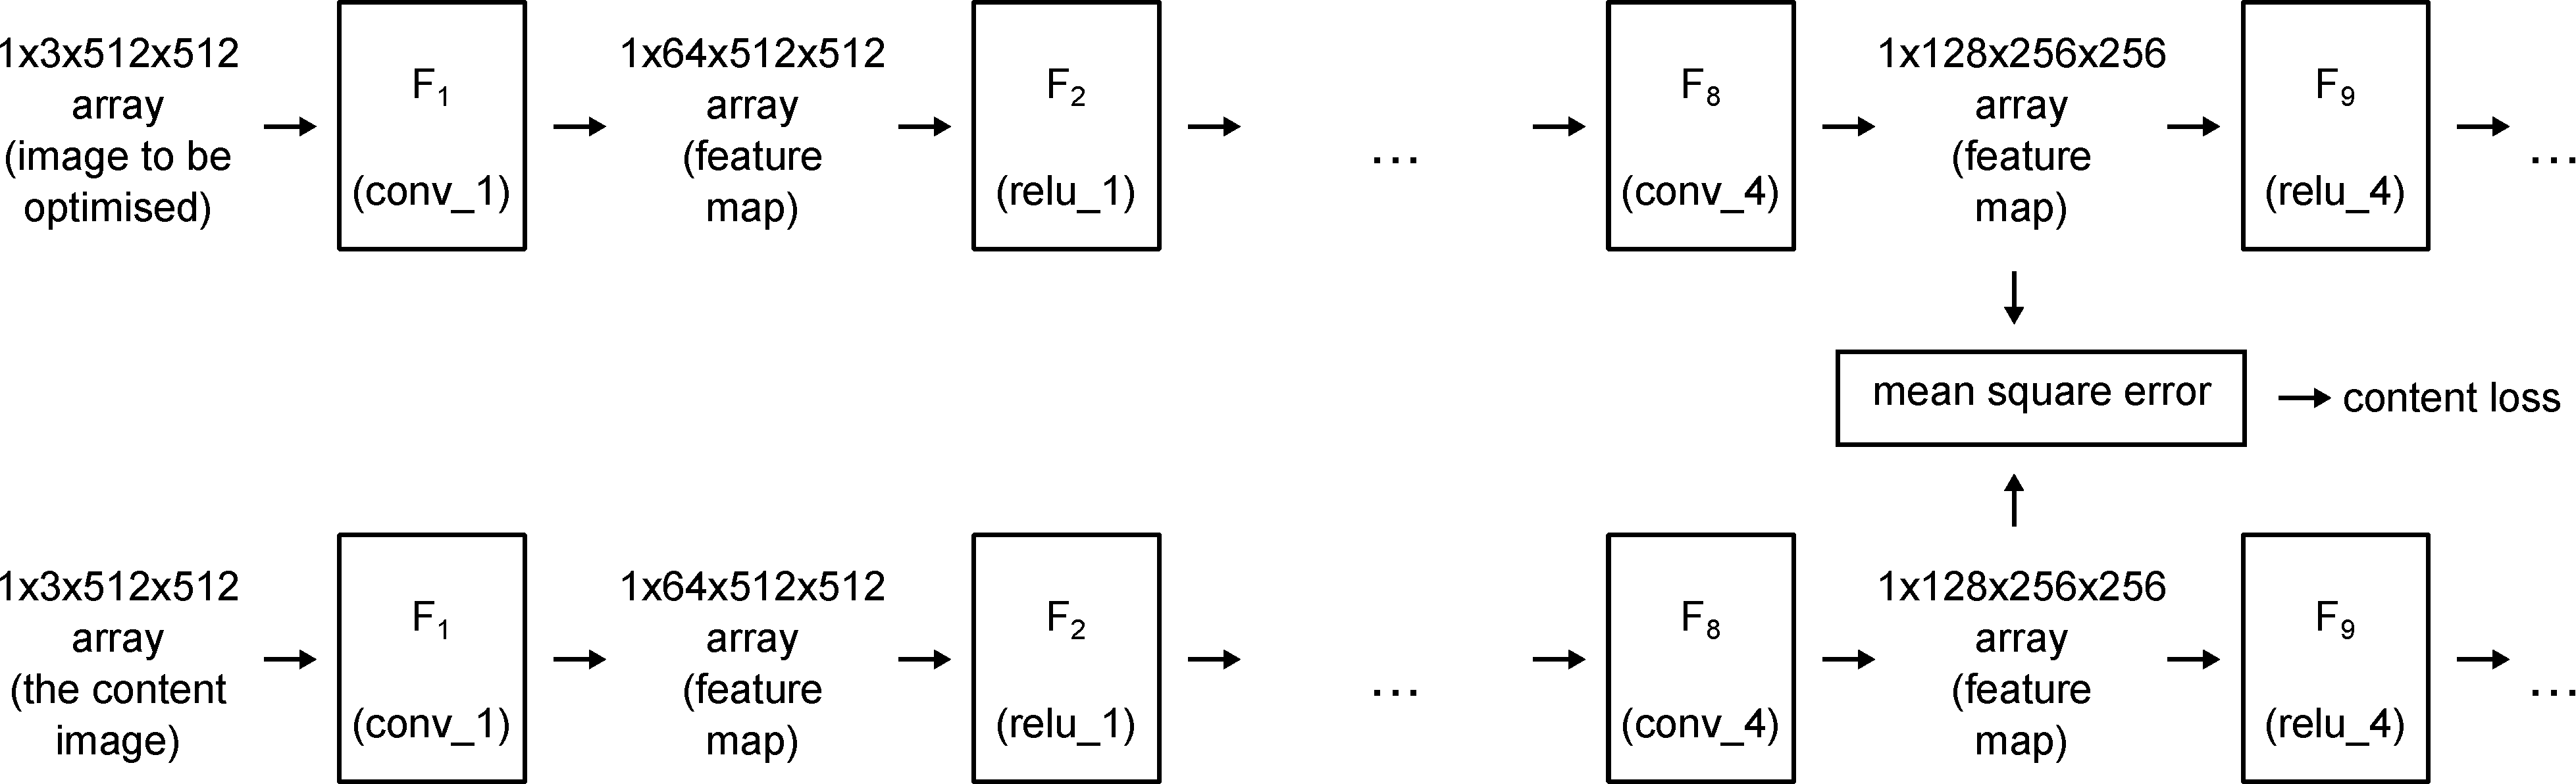
\includegraphics[width=\textwidth]{contentloss.pdf}
\caption{The content loss \label{contentloss}}
\end{figure}


The style loss $L_\text{content}$ can actually be a sum of several style losses, or sometimes just one.
For each style loss, 
both the current image under optimisation and the style image are passed through the vgg19 model.
The two outputs of a certain function in the model are extracted, 
and converted to Gram matrices. We will elabrate on what Gram matrices are later.
For now a Gram matrix is just a square matrix computed from a multidimensional array (i.e. a feature map).
For example, the Gram matrix (in the style transfer algorithm) of a $1\times64\times512\times512$ array
is a $64\times64$ matrix.
The point is that a Gram matrix describes the distribution of features
in the image without the spatial information of where the features are.
Gram matrices describe the distribution with correlation between features.
The several style losses are computed with the outputs of different functions.
Otherwise, each of the several style losses are computed in exactly the same way.
Again, the outputs of which functions in the model to derive style losses from is really adjustable.
A nice default we used was \verb|conv_1|,\verb|conv_2|,...,\verb|conv_5|. We illustrate
the style losses derived from the output of \verb|conv_1| in Figure $\ref{styleloss}$.

\begin{figure}
\center
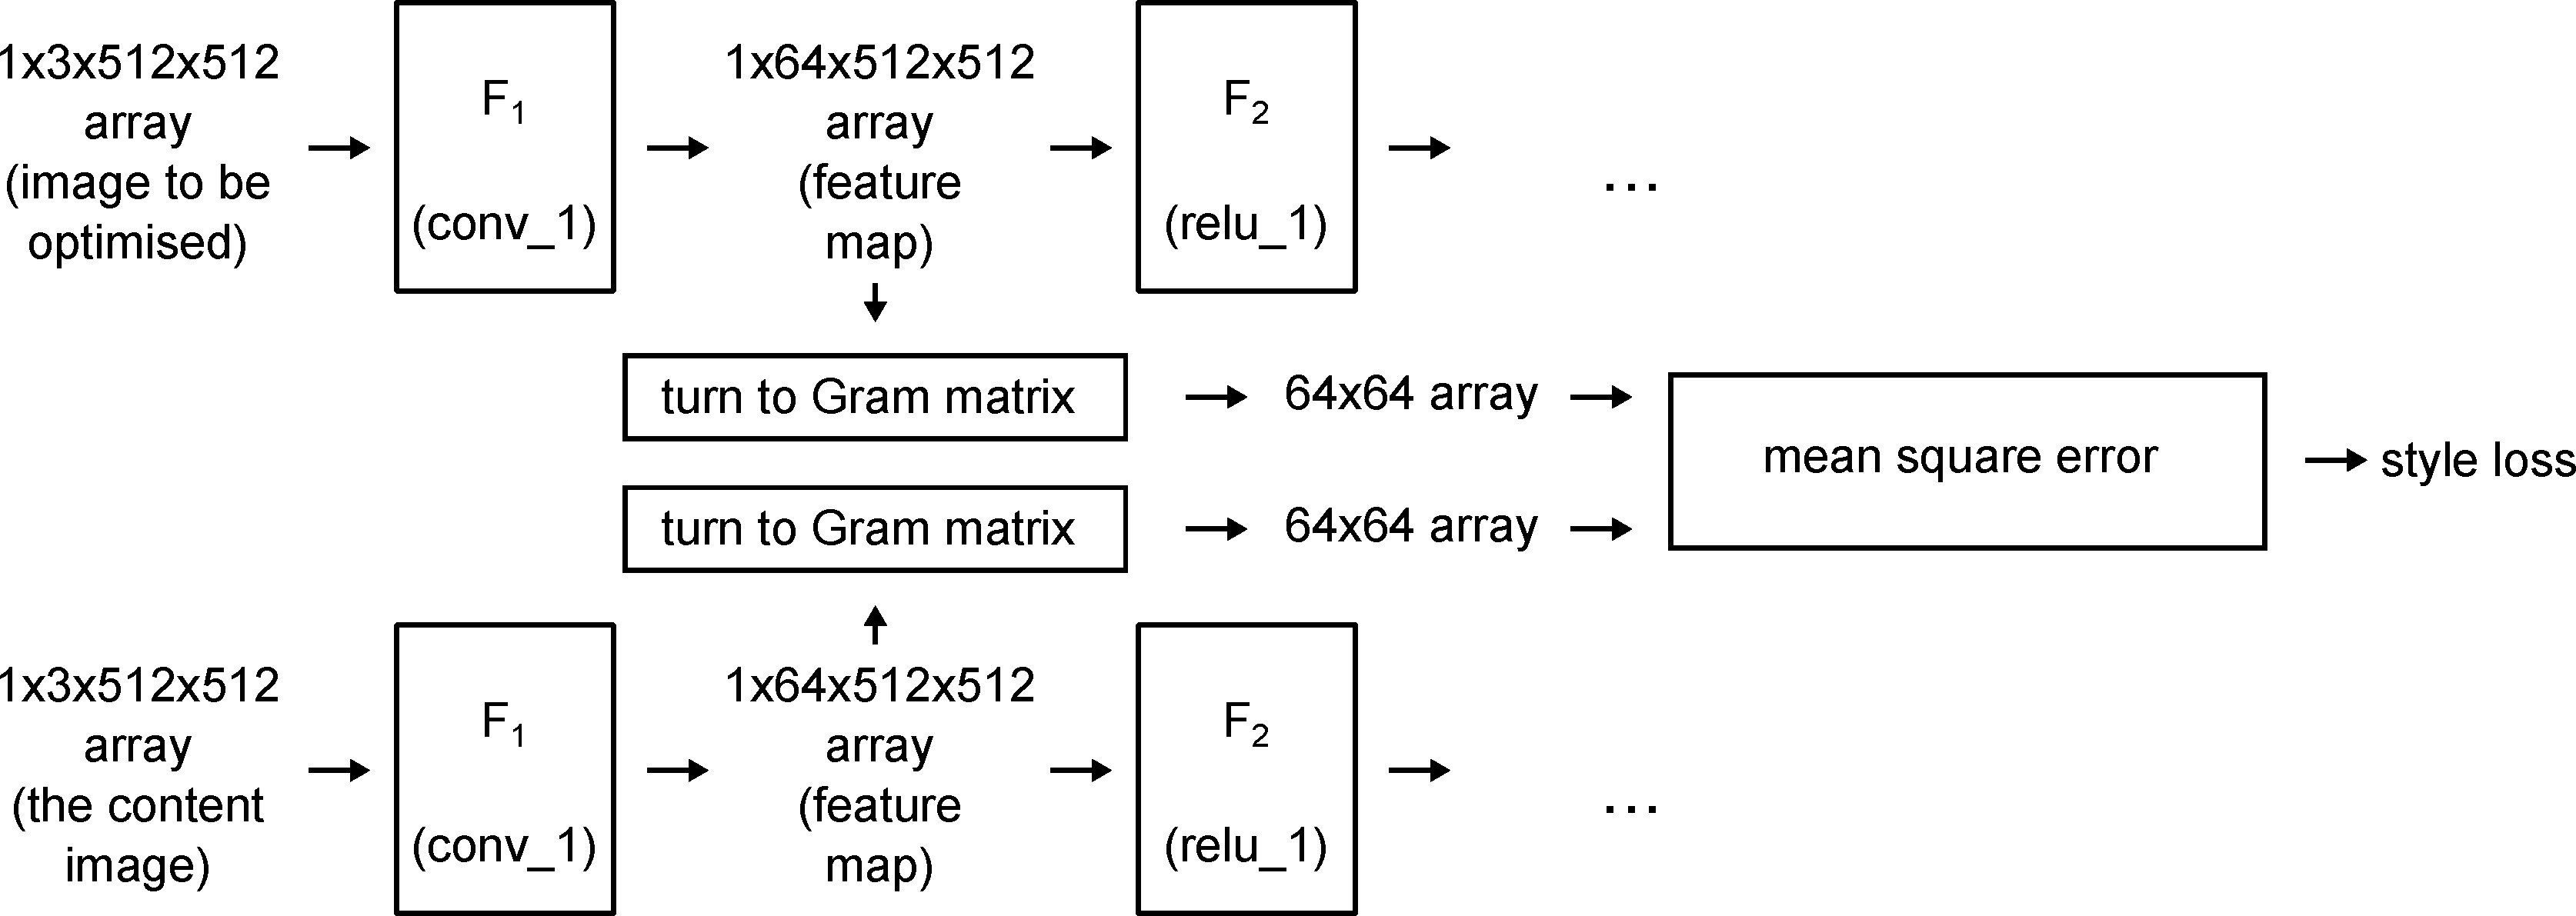
\includegraphics[width=\textwidth]{styleloss.pdf}
\caption{The style loss derived from the output of conv\_1 \label{styleloss}}
\end{figure}

\subsection{Gram matrix}
Gram matrix is responsible for extracting the style of an image by specifically computing the style loss 
from the style image. For Gram matrix computation, feature vectors are flattened for efficient computation 
that could be easily explained with the help of dot products where more similar the vectors are, lesser the 
angle of difference between them indicating the closer feature relation between image vectors. More angle of 
difference indicates the varied feature image vectors.By computing the dot product of all convolutional 
feature maps with every other feature map yields Gram Matrix which is formulated as, 




\subsection{Removing the spatial information in other ways}
We think that the most brilliant aspect of the neural style transfer algorithm,
apart from the general structure, is the use of Gram matrices to compare 
distributions of features in two images, so that where the features are does not matter.
It gives really nice insight on what ``artistic style'' means.

Now we wonder, could we achieve similar results with other ways to compare 
distribution of features?
One approach would be to consider the \emph{comparison} as a whole to find 
substitutes. 
For example, minimising the mean square errors between two Gram matrices could be seen as 
a special case for minimising a Maximum Mean Discrepancy (MMD), which means other Maximum Mean Discrepacies
could be used \cite{MMD}.
Maximum Mean Discrepancy is the spatial probability measure distance that has enormous applications in 
non-parametric testing and machine learning domain. It is defined as the distance between the neighbouring 
mean elements in probability space. 

MMDk(P, Q)=||μP * μQ||H Where μ is  the mean in the probability measure space.

For us, it seemed more natural to consider substitutes for the process itself of 
transforming a feature map into a Gram matrix. 
That is, we will consider other
mappings that remove the spatial information or where features are in a feature map but retain
the distribution of features, like a histogram.
Such functions need to be differentiable as well, otherwise they would render the 
optimisation infeasible.

We will call such functions ``\emph{dislocators}'' in the remaing part of this work.
Unfortunately, the word ``dislocate'' would give the connotation of moving something to somewhere else.
Nevertheless, the word ``locator'' means something that provides spatial information,
so calling somthing that removes spatial information a ``dislocator'' is still reasonable.

Other ``dislocator'' functions whose output somehow describe the 
distribution of features in their input should then work as substitutes
for computing Gram matrices.
The first few simplistic ``dislocator'' functions we tried are listed here.
\begin{enumerate}
\item Scaled sum of the responses all over the place for each feature.
That is, for an $1\times64\times256\times256$ feature map,
we compute an $1\times64$ array where each element is the sum of the
$256\times256$ elements from the input.
The whole array is then scaled to one over the total number of elements of the input feature map.
\item Scaled sum of element-wise squares of the responses over the place for each feature.
Other than an additional element-wise squaring, it is identical to the previous one.
\item Scaled sum of absolute values of the responses over the place for each feature.
\end{enumerate}

To find more dislocators, let us consider \emph{how to describe a distribution} in general?
The obvious answer is then sample statistics or estimators, like (sample) mean, (sample) standard deviation, 
(sample) skewness, (sample) kurtosis and any moments.
Unfortunately, we found that higher moments are too slow to compute for experiments,
so we ended up with the following (combinations) of sample statistics.
%\begin{enumerate}
%\end{enumerate}



\section{Experiments and Discussion}

\subsection{Reproducing the original result}

\subsection{Varying the dislocator function}

\subsection{Varying the extraction points for losses}

We will also show that other factors, such that the outputs of which functions to derive the style 
losses from are not very essential and somewhat belongs to tuning.

\section{Conclusion}
We have successfully implemented neural style transfer and generated the blende pastiche image
using content image and style image. We have finally concluded that Artistic image is created
with the help of pre-trained CNN. we did use vgg-19 model which is pre-trained model for object 
and face detection and we saw how effectively it was able to detect the texture,and contour of
the image. We determine the content loss by selecting a particular hidden layer’s activation. 
We also determined the style loss with help of Gram Matrix of the hidden layer’s activations.
Total style loss was computed by summing up all the style loss till the layers from where the
content image is selected. Losses were evaluated by using gradient loss dynamically. This was
computed using optimization algorithm of Broyden–Fletcher–Goldfarb–Shanno. This was done by 
inputting the every iteration loss to the network.

\section{Observation}
We found out that we can modify how much style of style image can be inserted in the final image. 
In order to do this, we determined how much content and style of the content image and style image
need to be present. These can be used as hyper parameters to develop the final artistic image. 
More weights of the style of the style image leads to more style and content of the style image
are going to be present in the generated image vice-versa. Another hyper parameter is to choose
the CNN hidden layer activation for the content image. This helps to decide how much content
of content images needs to present in the generated image.

\section{Discussion}
We did find that by putting more weights to style image, more style and content of style images
were getting displayed. By putting in the context, when weights are 105  then content and style
of the content image is lost and style of style image is on the generated image but content of
style image was distorted. In the another process, we did choose different hidden activation layer
in CNN for content image. Ideally, we have selected the middle layer which is ‘CONV_4’. We can
select any of convolution layer to see different result. We found out that by selecting the CONV_1,
the textures of the content image are more prominent. We also found it amazing that after the certain
number of iterations, we are getting blacked out image. It could be possible that losses would have
become zero in this case which further altering the pixel values of the image. However, this is 
something need to be researched Thoroughly.

\section{Lessons Learnt}
We were able to use Pytorch and Tensorflow libraries to implement the image stylization.
We also understood how well CNN model works when image is given as input. We learned to 
compute difference between the two images with the help of content and style. This can be 
computed with the help of gradient loss.


\section {Future Work}
At present, we are applying style of the style image to the whole content image. We are thinking
of using image segmentation technique[1] so to apply style on a particular segment of the image. 
For example, there is a photograph of person wearing a jacket, applying this new technique, 
we would style the jacket with help of some art and apply it back to original image. This means 
old jacket becomes the new one.

\section{Summary of Learning Outcome} 
We learned some crucial concept of programming the project in python using pyTorch and Tensorflow. 
We analysed and evaluated neural style transfer algorithm. We also learned to examined the research
paper and how to link the research paper with other researches to form an innovation solutions. 
We also learned to work in a team. We were able to reflect and use the course learning as our future
work for the neural style transfer.


\begin{thebibliography}{8}
\bibitem{nst}
Gatys, L., Ecker, A., \& Bethge, M. (2016). A neural algorithm of artistic style. Journal of Vision, 16(12), 326. doi:10.1167/16.12.326
\bibitem{MMD}
Li, Y., Wang, N., Liu, J., \& Hou, X. (2017). Demystifying Neural Style Transfer. IJCAI.
\bibitem{interp}
Doshi-Velez, F., \& Kim, B. (2017). Towards A Rigorous Science of Interpretable Machine Learning.
\bibitem{pytorch}
Paszke, A., Gross, S., Chintala, S., Chanan, G., Yang, E., DeVito, Z., Lin, Z., Desmaison, A., Antiga, L., \& Lerer, A. (2017). Automatic differentiation in PyTorch.
\end{thebibliography}
\end{document}

